\documentclass[border=12pt]{standalone}
\def\pgfsysdriver{pgfsys-dvisvgm.def}
\usepackage[dvisvgm]{xcolor}
\usepackage{xeCJK}
\setCJKmainfont{HaranoAjiGothic-Regular.otf}[BoldFont=HaranoAjiGothic-Bold.otf]
\setCJKsansfont{HaranoAjiGothic-Regular.otf}[BoldFont=HaranoAjiGothic-Bold.otf]
\usepackage{amsmath,amssymb,tikz,lmodern}
\usetikzlibrary{arrows.meta,positioning,calc,fit,backgrounds}
\renewcommand{\familydefault}{\sfdefault}
\definecolor{ink}{HTML}{25322F}
\definecolor{green}{HTML}{246657}
\definecolor{tint}{HTML}{EEF4F0}
\definecolor{soft}{HTML}{C6D2CC}
\definecolor{muted}{HTML}{52615B}
\newif\ifJapanese
\newcommand{\Tx}[2]{\ifJapanese #1\else #2\fi}
\newcommand{\Eff}{\overline{\operatorname{Eff}}}
\newcommand{\heading}[3]{{\color{green}\bfseries #1\quad\Tx{#2}{#3}}\\[5pt]}
% A white rectangle makes the complete citation label clickable, including spaces.
\newcommand{\refurl}[2]{\special{dvisvgm:raw <a xlink:href="#1" target="_blank" rel="noopener noreferrer">}{\setlength{\fboxsep}{0pt}\colorbox{white}{\color{green}\underline{\strut #2}}}\special{dvisvgm:raw </a>}}
\tikzset{
 card/.style={draw=soft,fill=white,rounded corners=2pt,align=left,text=ink,font=\fontsize{10.5}{14}\selectfont,inner xsep=12pt,inner ysep=10pt,text width=14.4cm},
 half/.style={card,text width=6.45cm,minimum height=2.05cm},
 result/.style={card,draw=green,fill=tint,line width=.9pt},
 reason/.style={align=left,text=muted,font=\fontsize{9}{12}\selectfont,inner sep=0pt,text width=12.7cm},
 branchreason/.style={reason,text width=5.95cm},
 edge/.style={-{Stealth[length=2.4mm]},draw=green,line width=1pt},
 wire/.style={draw=green,line width=1pt},
}
% Keep the arrow in a dedicated left gutter; explanations never cover it.
\newcommand{\flow}[3]{
 \coordinate (#2-from) at ($(#1.south)+(-6.9,0)$);
 \coordinate (#2-to) at ($(#2.north)+(-6.9,0)$);
 \draw[edge] (#2-from)--(#2-to);
 \node[reason,anchor=west] (#2-reason) at ($(#2-from)!.5!(#2-to)+(.55,0)$) {#3};
}

\newcommand{\Cite}[2]{\refurl{#1}{#2}}

\Japanesetrue
\begin{document}
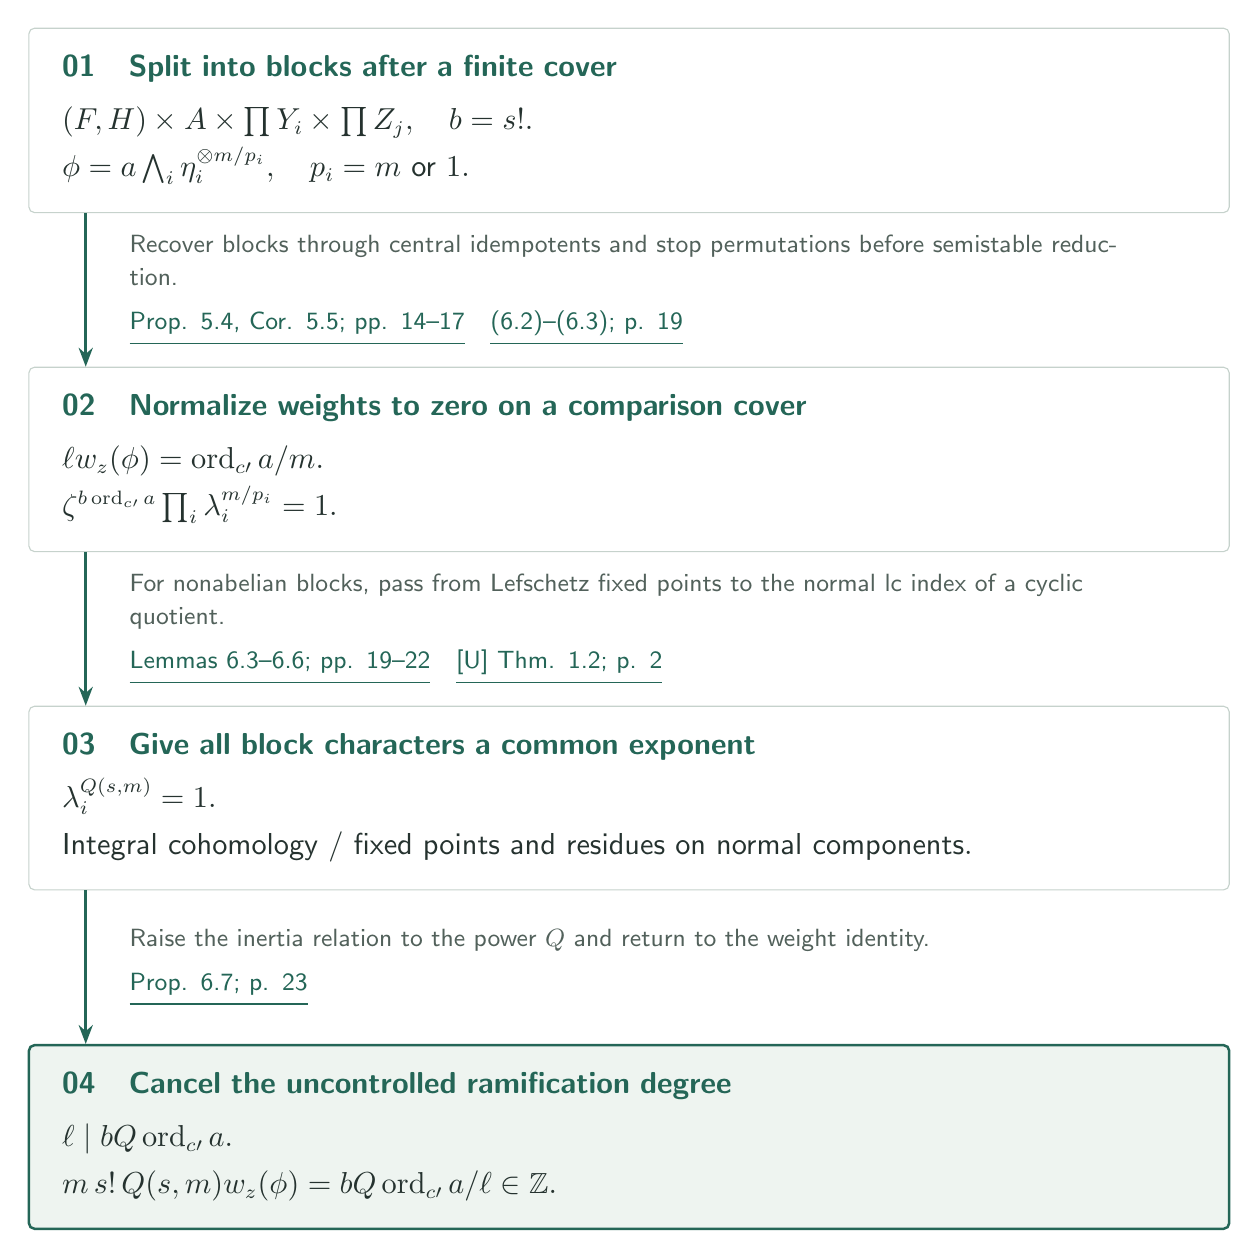
\begin{tikzpicture}
\node[card] (n0) {\heading{01}{有限被覆上で境界付きブロックに分解}{Split into blocks after a finite cover}$(F,H)\times A\times\prod Y_i\times\prod Z_j,\quad b=s!.$\\[3pt] $\phi=a\bigwedge_i\eta_i^{\otimes m/p_i},\quad p_i=m\text{ or }1.$};
\node[card,below=1.95cm of n0] (n1) {\heading{02}{比較被覆上で重みを0に正規化}{Normalize weights to zero on a comparison cover}$\ell w_z(\phi)=\operatorname{ord}_{c\prime}a/m.$\\[3pt] $\zeta^{b\operatorname{ord}_{c\prime}a}\prod_i\lambda_i^{m/p_i}=1.$};
\flow{n0}{n1}{\Tx{中心冪等元でブロックを回復し、置換を止めてから半安定化。}{Recover blocks through central idempotents and stop permutations before semistable reduction.}\\[4pt]\Cite{https://github.com/openai/math/blob/adc7f1241b42e322a6451854ab7e4b4c146bf78a/preprints/Uniform-log-Iitaka-fibrations-and-bounded-moduli-denominators-October-4-2026/uniform-log-iitaka.pdf}{Prop. 5.4, Cor. 5.5; pp. 14--17}\quad \Cite{https://github.com/openai/math/blob/adc7f1241b42e322a6451854ab7e4b4c146bf78a/preprints/Uniform-log-Iitaka-fibrations-and-bounded-moduli-denominators-October-4-2026/uniform-log-iitaka.pdf}{(6.2)--(6.3); p. 19}}
\node[card,below=1.95cm of n1] (n2) {\heading{03}{各ブロックの指標に共通の指数を与える}{Give all block characters a common exponent}$\lambda_i^{Q(s,m)}=1.$\\[3pt] $\Tx{\text{整コホモロジー / 固定点と正規成分への留数}}{\text{Integral cohomology / fixed points and residues on normal components}}.$};
\flow{n1}{n2}{\Tx{非アーベル成分ではLefschetzの固定点から巡回商のnormal lc指数へ。}{For nonabelian blocks, pass from Lefschetz fixed points to the normal lc index of a cyclic quotient.}\\[4pt]\Cite{https://github.com/openai/math/blob/adc7f1241b42e322a6451854ab7e4b4c146bf78a/preprints/Uniform-log-Iitaka-fibrations-and-bounded-moduli-denominators-October-4-2026/uniform-log-iitaka.pdf}{Lemmas 6.3--6.6; pp. 19--22}\quad \Cite{https://github.com/openai/math/blob/adc7f1241b42e322a6451854ab7e4b4c146bf78a/preprints/Uniform-Pluricanonical-Iitaka-Fibrations-October-3-2026/paper.pdf}{[U] Thm. 1.2; p. 2}}
\node[result,below=1.95cm of n2] (n3) {\heading{04}{制御しない分岐次数を消去する}{Cancel the uncontrolled ramification degree}$\ell\mid bQ\operatorname{ord}_{c\prime}a.$\\[3pt] $m\,s!\,Q(s,m)w_z(\phi)=bQ\operatorname{ord}_{c\prime}a/\ell\in\mathbb Z.$};
\flow{n2}{n3}{\Tx{慣性群の関係式を $Q$ 乗し、重みの式へ戻す。}{Raise the inertia relation to the power $Q$ and return to the weight identity.}\\[4pt]\Cite{https://github.com/openai/math/blob/adc7f1241b42e322a6451854ab7e4b4c146bf78a/preprints/Uniform-log-Iitaka-fibrations-and-bounded-moduli-denominators-October-4-2026/uniform-log-iitaka.pdf}{Prop. 6.7; p. 23}}
\end{tikzpicture}

\end{document}
